\section{سوال سوم}
برای بهینه‌سازی از روش
\lr{SA}
استفاده شده است.
تابع دما به صورت زیر در نظر گرفته شده است.
$$
T_{k+1} = \alpha T_{k}
$$

در اجرای کد دو حالت ۱۰ و ۱۰۰  زنجیره مارکو در اجرا شده است و نتایج در جدول
\ref{tab:result}
آورده شده است. برای یافتن همسایگی از عوض کردن خانه‌های رشته جواب استفاده شده است. تعداد خانه‌های عوض شده تابعی از دما است. به این صورت، از حداکثر ۴ خانه تا حداقل ۲ خانه انجام شده است. پارامتر‌های انتخاب شده برای بهینه‌سازی با
\lr{random sampling}
شامل دمای اولیه، دمای نهایی و ضریب $\alpha$ است.
بازه جواب‌ها در جدول \ref{tab:parameters} آمده است.

\lr{\begin{table}[!h]
		\caption{Parameter of SA algorithm}
		\vspace{0.5cm}
		\centering
		\begin{tabular}{|c|c|c|c|}
			\hline
			 $\alpha$ & $T_f$ & $T_0$  &  Parameter
			\\ \hline
			$0.99$ & $10^0$ & $10^5$ & $\max$ \\
			$0.90$ & $10^{-4}$ & $10^2$ & $\min$
 		  \\ \hline
		\end{tabular}
	\label{tab:parameters}
\end{table}}



\begin{table}[!h]
		\caption{نتایج اجرا با مجموعه‌های مختلف}
		\vspace{0.5cm}
		\centering
		\begin{tabular}{|c|c|c|c|}
			\hline
			\lr{Set 3} & \lr{Set 2} & \lr{Set 1}  &  نتایج
			\\ \hline
			$20$ & $20$ & $20$ &
			 تعداد اجراهای موفق \\
		$125.5$ & $124.7$ & $122.1$ &
		 میانگین کمترین زمان امدادرسانی\\
				$6791$ & $8497$ & $7805$ &
				 میانگین تعداد ارزیابی تا نخستین دستیابی به بهترین جواب
			\\ \hline
		\end{tabular}\label{tab:result}
\end{table}

نمودار دما بر حسب تابع هزینه برای بهترین پارامتر‌های بدست آمده رسم شده است.


\begin{figure}[H]
	\caption{نتایج الگوریتم \lr{SA} در کل دماها} 
	\centering 
	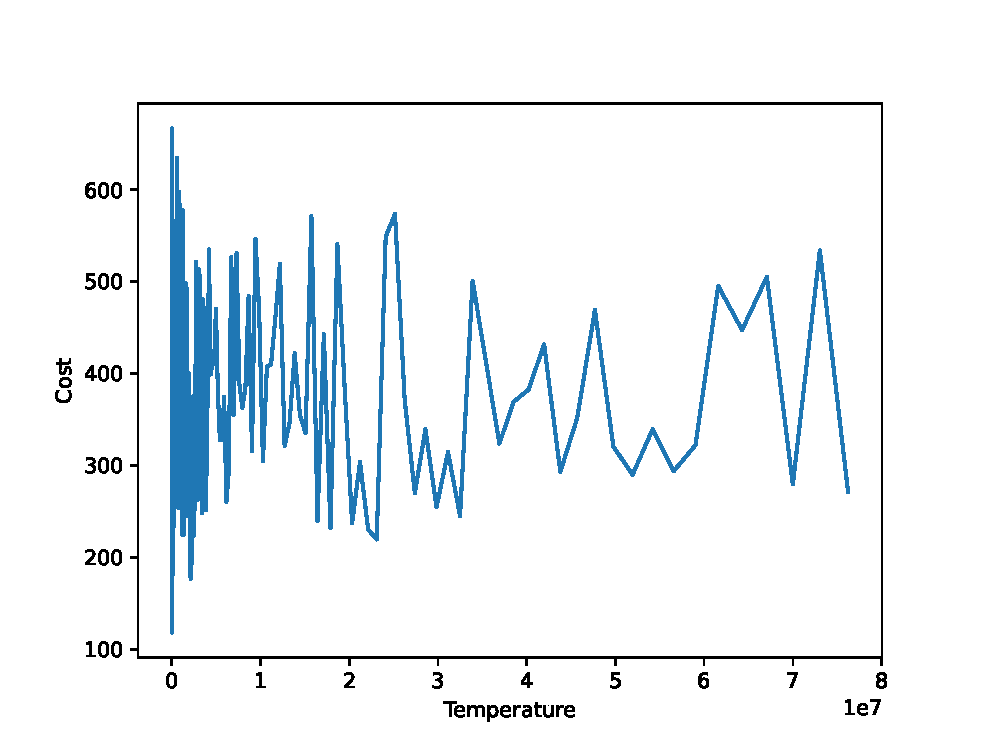
\includegraphics[width=12cm]{../Figure/Q3/all} 
\end{figure}

\begin{figure}[H]
	\caption{نتایج الگوریتم \lr{SA} در دماهای نزدیک به صفر} 
	\centering 
	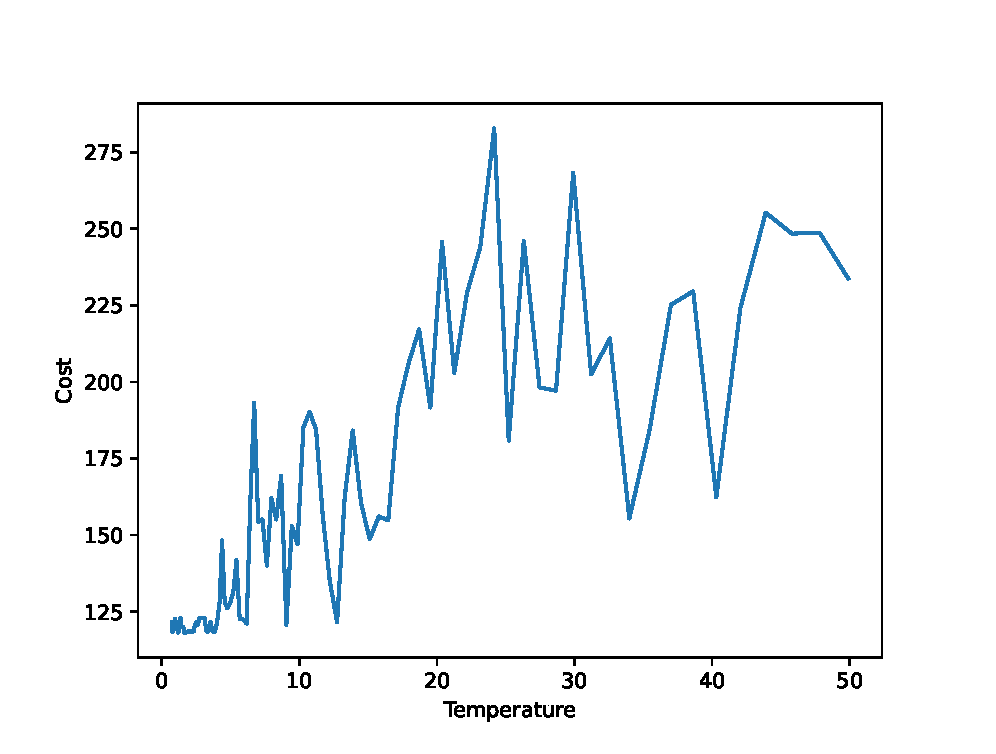
\includegraphics[width=12cm]{../Figure/Q3/final} 
\end{figure}



